\begin{figure}[H]
\begin{center}
\beginpgfgraphicnamed{plot_HP2.pdf}
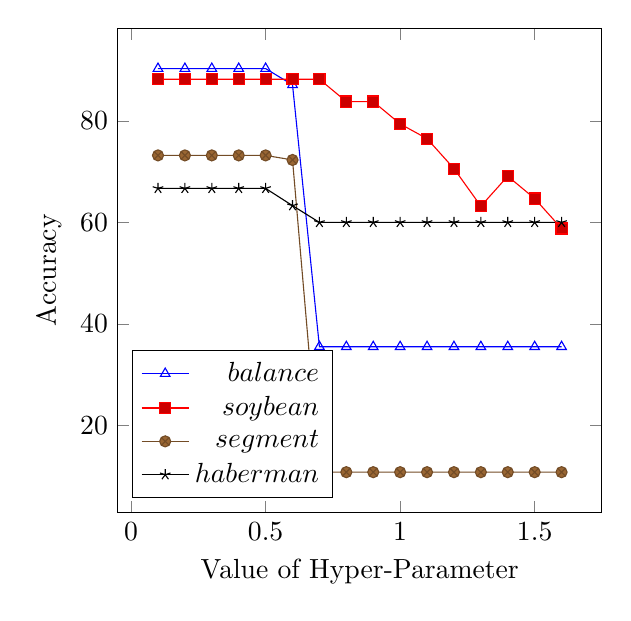
\begin{tikzpicture}
\centering
\begin{axis}
[ylabel=Accuracy,
xlabel=Value of Hyper-Parameter,
width=220pt,
height=220pt,
legend style={
	cells = {anchor = east},
	legend pos = south west,
	},
]
\addplot+[sharp plot, mark=triangle] coordinates
        {(0.1,90.3) (0.2,90.3) (0.3,90.3) (0.4,90.3) (0.5,90.3) (0.6,87.1) (0.7,35.5) (0.8,35.5) (0.9,35.5) (1.0,35.5) (1.1,35.5) (1.2,35.5) (1.3,35.5) (1.4,35.5) (1.5,35.5) (1.6,35.5)};
\addplot+[sharp plot] coordinates
        {(0.1,88.2) (0.2,88.2) (0.3,88.2) (0.4,88.2) (0.5,88.2) (0.6,88.2) (0.7,88.2) (0.8,83.8) (0.9,83.8) (1.0,79.4) (1.1,76.5) (1.2,70.6) (1.3,63.2) (1.4,69.1) (1.5,64.7) (1.6,58.8) };
\addplot+[sharp plot] coordinates
        {(0.1,73.2) (0.2,73.2) (0.3,73.2) (0.4,73.2) (0.5,73.2) (0.6,72.3) (0.7,10.8) (0.8,10.8) (0.9,10.8) (1.0,10.8) (1.1,10.8) (1.2,10.8) (1.3,10.8) (1.4,10.8) (1.5,10.8) (1.6,10.8)};
\addplot+[sharp plot] coordinates
        {(0.1,66.7) (0.2,66.7) (0.3,66.7) (0.4,66.7) (0.5,66.7) (0.6,63.3) (0.7,60.0) (0.8,60.0) (0.9,60.0) (1.0,60.0) (1.1,60.0) (1.2,60.0) (1.3,60.0) (1.4,60.0) (1.5,60.0) (1.6,60.0)};
        
\legend{$balance$,$soybean$,$segment$,$haberman$}
\end{axis}
\end{tikzpicture}
\endpgfgraphicnamed
\end{center}
\caption{Influence of HyperParameter tuning on Classification Accuracy 2}
\end{figure}